\documentclass[11pt,a4paper]{article}
\usepackage[left=2cm,right=2cm,top=2cm,bottom=2cm]{geometry}
\usepackage{xcolor}
\usepackage{hyperref}
\usepackage{titlesec}
\usepackage{graphicx}
\usepackage{enumitem}
\usepackage{tabularx}

\hypersetup{
  colorlinks=true,
  linkcolor=blue,
  urlcolor=blue
}

\titleformat{\section}{\Large\bfseries}{}{0em}{}[\titlerule]
\setlist[itemize]{leftmargin=*, itemsep=0.25em}

\begin{document}

\begin{minipage}[t]{0.70\textwidth}
{\huge\bfseries Curriculum Vitae}\\[0.5cm]
{\Large\bfseries Sangdon Park}\\[0.2cm]
Assistant Professor, Department of Computer Engineering\\
School of SW Convergence, Daejeon University\\
(Appointed: 2026.03.01)\\[0.25cm]
\href{mailto:sangdon.park@dju.kr}{sangdon.park@dju.kr}\\
\href{https://sangdon-park.github.io}{https://sangdon-park.github.io}\\
\href{https://scholar.google.com/citations?user=JZFDtsgAAAAJ}{Google Scholar} \quad
\href{https://github.com/Sangdon-Park}{GitHub} \quad
\href{https://www.linkedin.com/in/sangdon/}{LinkedIn}
\end{minipage}%
\hfill
\begin{minipage}[t]{0.27\textwidth}
\begin{flushright}
\IfFileExists{images/Sangdon.jpg}{
  
\includegraphics[width=0.8\textwidth]{images/Sangdon.jpg}
}{
  \IfFileExists{../images/Sangdon.jpg}{
    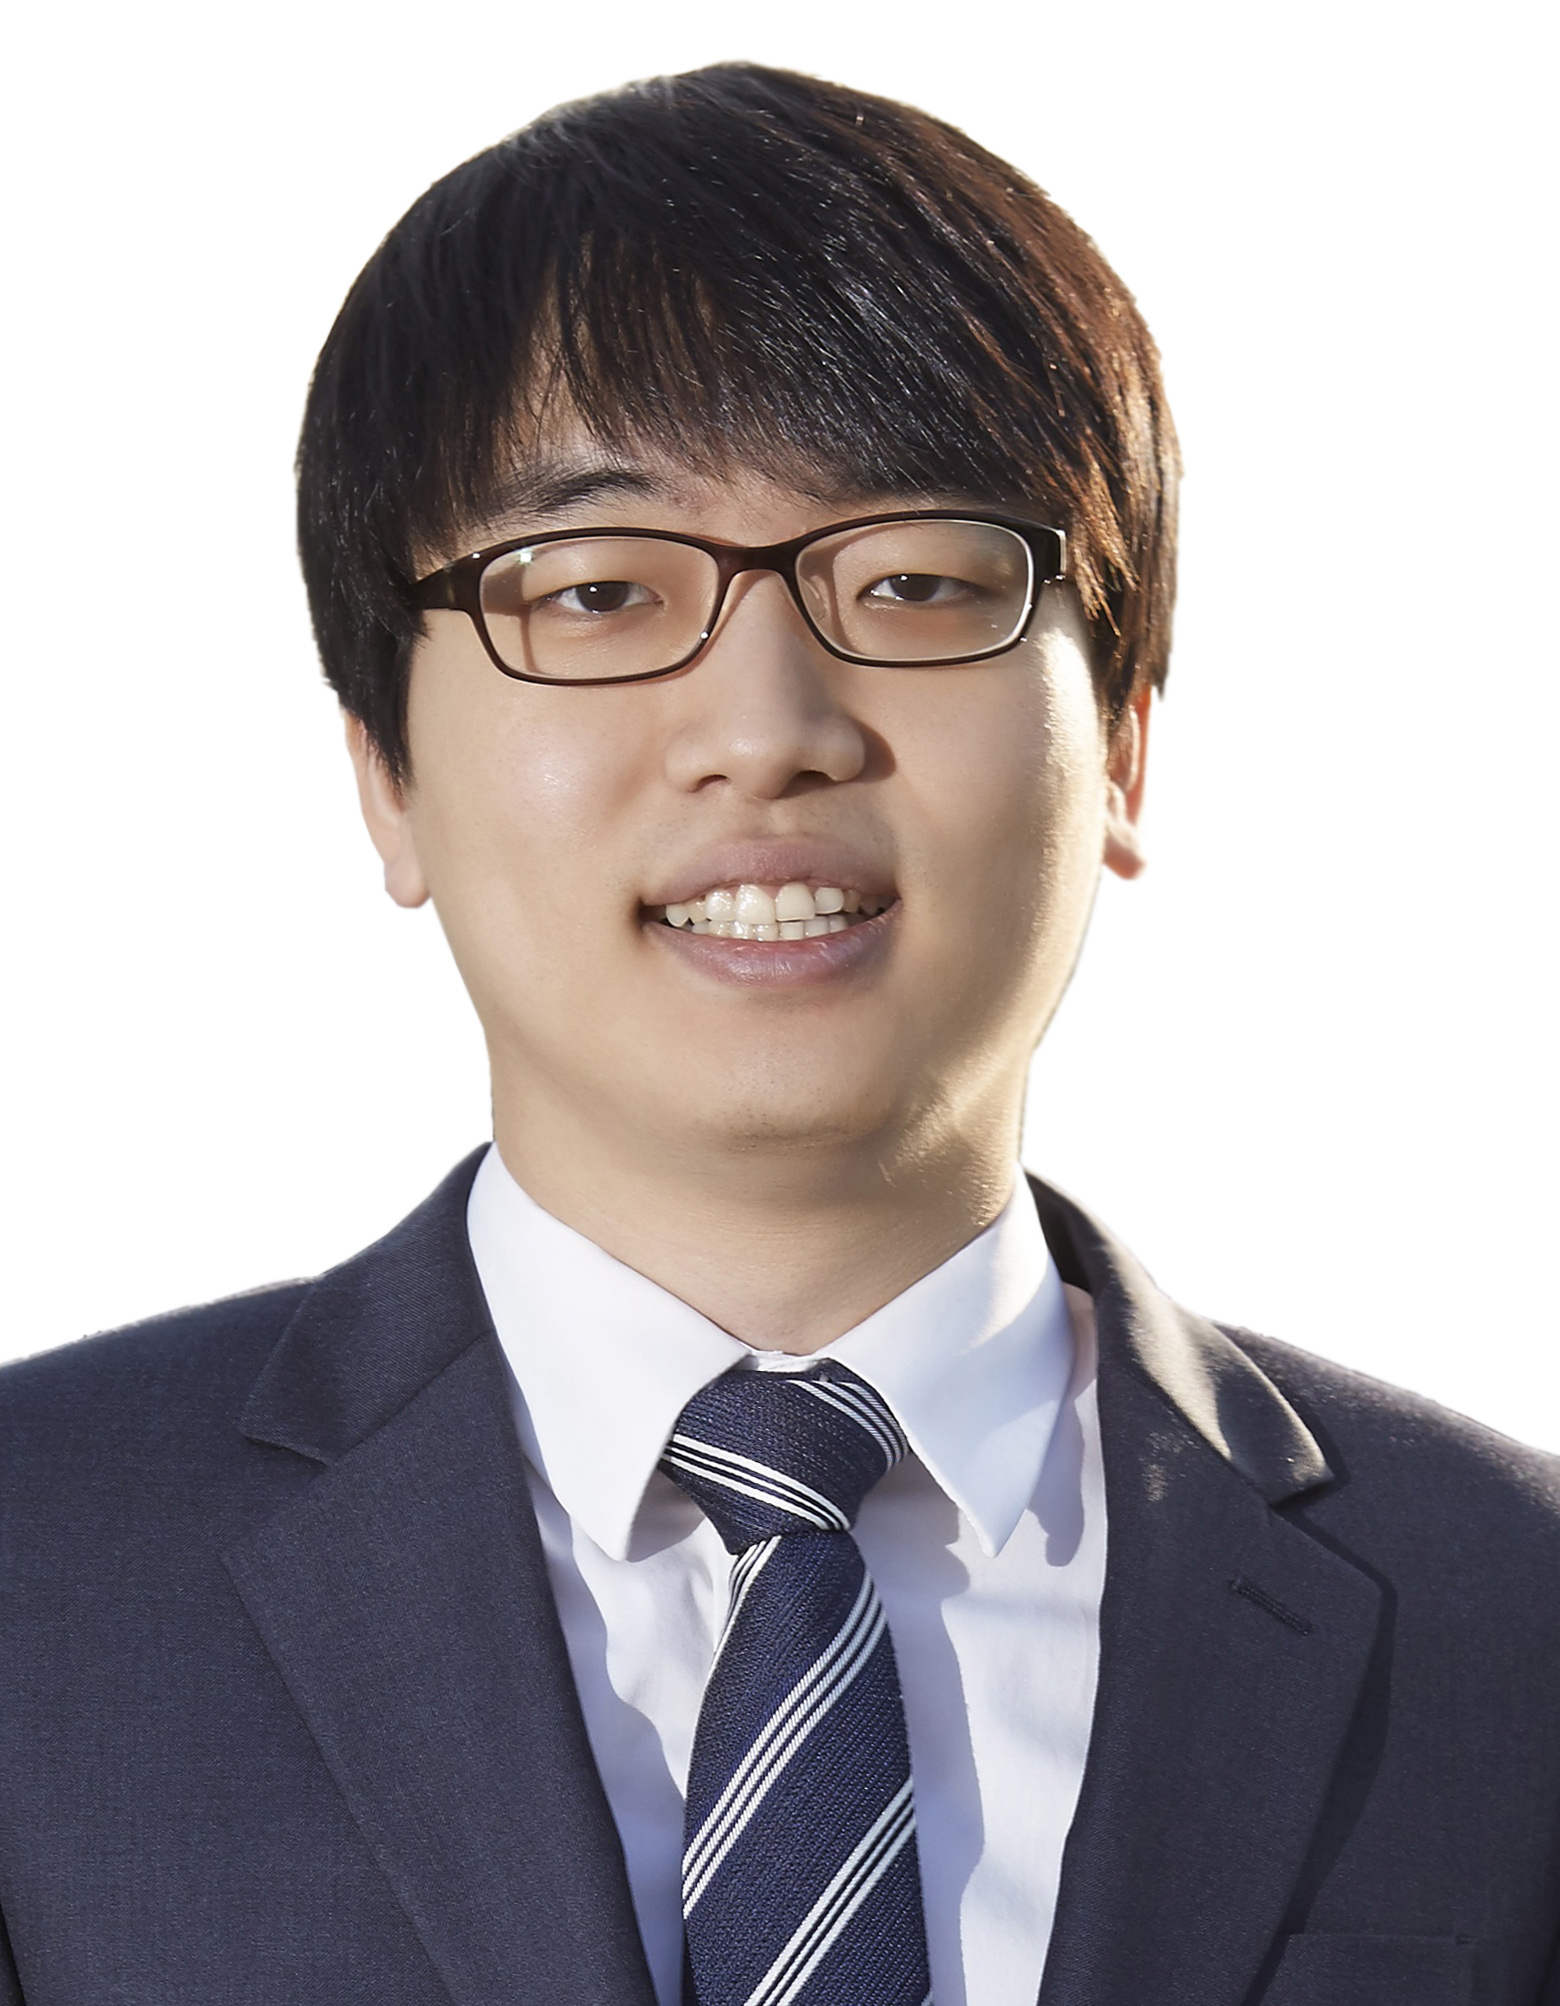
\includegraphics[width=0.8\textwidth]{../images/Sangdon.jpg}
  }{}
}
\end{flushright}
\end{minipage}

\section{Research Profile}
\begin{itemize}
  \item AI x Games Systems
  \item Edge/network resource optimization and dynamic pricing
  \item AI/LLM systems (RAG, tool-use, agent evaluation)
  \item Interactive AI applications and game development
\end{itemize}

\section{Appointments}
\begin{tabularx}{\textwidth}{Xr}
\textbf{Assistant Professor}, Department of Computer Engineering, School of SW Convergence, Daejeon University & 2026.03.01 -- Present \\
\textbf{Game Developer}, Sayberry Games & 2025.05 -- 2026.02.28 \\
\textbf{Postdoctoral Researcher}, KAIST Institute for Information Electronics Research (IIER) & 2017.09 -- 2025.04 \\
\end{tabularx}

\section{Education}
\begin{tabularx}{\textwidth}{Xr}
\textbf{Ph.D.}, School of Electrical Engineering, KAIST \newline
Advisor: Prof. Jun Kyun Choi & 2017.08 \\
\textbf{M.S.}, Department of Mathematical Sciences, KAIST \newline
Advisor: Prof. Ganguk Hwang & 2013.02 \\
\textbf{B.S.}, Department of Mathematical Sciences, KAIST & 2011.02 \\
\end{tabularx}

\section{Teaching (2026 Spring)}
\begin{itemize}
  \item Database Systems
  \item Artificial Intelligence
  \item Capstone Design
\end{itemize}

\section{Projects}
\begin{itemize}
  \item \textbf{Hexagon Soup} (solo development, in progress): \href{https://store.steampowered.com/app/4256880/Hexagon_Soup/}{Steam Page}
\end{itemize}

\section{Publications}
International Journals: 27 papers (4 first-authored, 13 corresponding-authored)\\
International Conferences: 10 papers (3 first-authored, 2 corresponding-authored)\\[0.2cm]

\textbf{Selected IEEE Journal Papers}
\begin{enumerate}[leftmargin=*]
  \item Sangdon Park, Sohee Bae, Joohyung Lee, Youngchul Sung, ``Real-Time Dynamic Pricing for Edge Computing Services: A Market Perspective,'' \textit{IEEE Access}, 2024.
  \item Hyeonseok Seo, Hyeontaek Oh, Jun Kyun Choi, Sangdon Park, ``Differential Pricing-Based Task Offloading for Delay-Sensitive IoT Applications in Mobile Edge Computing System,'' \textit{IEEE Internet of Things Journal}, 2022.
  \item Jaeseob Han, Gyeong Ho Lee, Sangdon Park, Jun Kyun Choi, ``Joint Subcarrier and Transmission Power Allocation in OFDMA-Based WPT System for Mobile-Edge Computing in IoT Environment,'' \textit{IEEE Internet of Things Journal}, 2022.
  \item Beomhan Baek, Joohyung Lee, Yuyang Peng, Sangdon Park, ``Three Dynamic Pricing Schemes for Resource Allocation of Edge Computing for IoT Environment,'' \textit{IEEE Internet of Things Journal}, 2020.
  \item Sangdon Park, Joohyung Lee, Sohee Bae, Ganguk Hwang, Jun Kyun Choi, ``Contribution-Based Energy-Trading Mechanism in Microgrids for Future Smart Grid: A Game Theoretic Approach,'' \textit{IEEE Transactions on Industrial Electronics}, 2016.
\end{enumerate}

Full publication list: \href{https://sangdon-park.github.io/publications.html}{https://sangdon-park.github.io/publications.html}

\end{document}
